The main complaint about patent search is an insufficient match between the content of patent queries and relevant
patents\cite{lupu2013patent}\cite{magdy2012toward}. However, considering the size of a patent query (usually thousand of words), the intuition is that there are enough terms to match the relevant patents. 
\subsection{Oracular Query Formulation}
We started with {\em relevance feedback} where we have access to the judged relevant documents. We calculate a relevance feedback (RF) score for each term in top-100 retrieved documents as follows:
\begin{equation}
score_{RF}(t,Q)=Rel(t)-Irr(t) 
 \label{eq:score}
\end{equation}\vspace*{-5ex}
\begin{displaymath}t\in \lbrace \mbox{terms in top-100 retrieved documents}\rbrace\end{displaymath}
where $ Rel(t) $ is the average term frequency in retrieved relevant patents and $ Irr(t) $ is the average term frequency in retrieved irrelevant patents. We assumed that words with a positive score are {\em useful words} since they are more frequent in relevant patents, while words with negative score are {\em noisy words} as they appear more frequently in irrelevant patents. 

We expected to see a higher performance for the queries which contain more {\em useful words}, but, surprisingly, we could not find any correlation between the performance and the presence of {\em useful words} in the query. 

We hypothesized that a query, formulated by only the {\em useful terms}, is the best possible query we can make since they are all frequent in relevant patents but rare in irrelevant ones. We formulated two oracular queries. The first query was formulated by positive terms in top-100 documents as follows: 
\begin{equation}
Oracular \; Query = \{t \in top-100|score_{RF}(t)>0\}   
 \label{eq:score}
\end{equation}
We formulated the second query by selecting only {\em useful terms} existing inside the patent query based on the hypothesis that a patent query contains sufficient words matched with the relevant patents:
\begin{equation}
 Oracular \; Patent \; Query = \{t\in Q|score_{RF}(t)>0\}   
 \label{eq:score}
\end{equation}
The system performance to these two queries were encouraging. We discuss the detailed results in the next section.

\subsection{Baseline vs. Oracular Query}
The system performed very well for both {\em Oracular Query} and {\em Oracle Patent Query}.  
\begin{table}[htpb]
  \begin{center}
   \caption{System performance for the {\em Patent Query}, {\em Oracular Query}, and {\em Best Run Query}.}
   \vspace*{1ex}
  \input table/optquery.tex   
  \label{tab:optquery}
  \end{center}  
\end{table}
As it can be seen in Table \ref{tab:optquery}, the {\em Oracular Query} far outperforms the baseline {\em Patent Query} and performs twice as well on MAP as the best competitor in CLEF-IP 2010~\cite{lopez2010experiments}.

We used a threshold $\tau$ to formulate the {\em Oracular Query} and {\em Oracular Query} to include merely terms with the RF score higher than $\tau$ ($score_{RF}(t,Q)>0$). 
\begin{figure}[htpb]
   \centering
   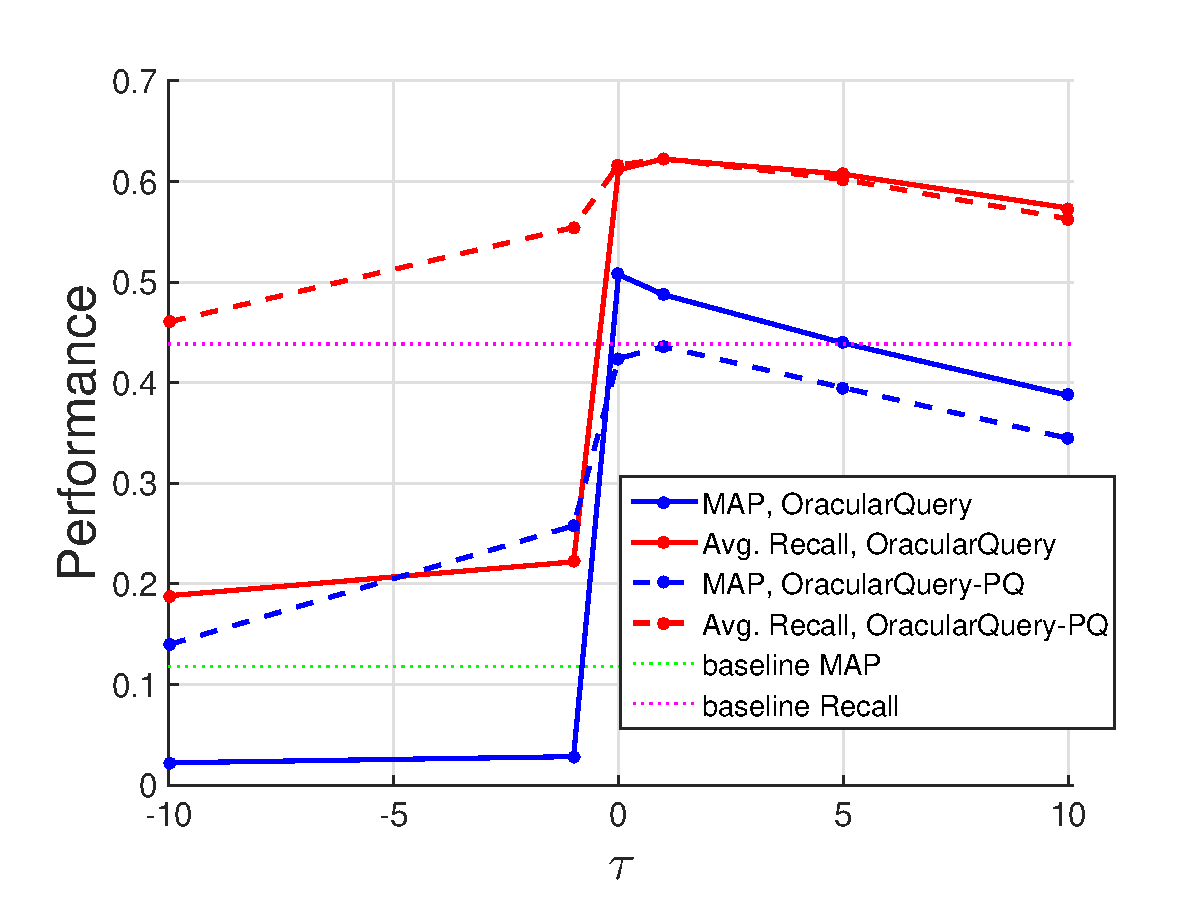
\includegraphics[width=0.35\textwidth,height=40mm]{figs/oracularquery1.eps}
   \caption{System performance vs. the threshold $\tau$ for oracular query and oracular patent query.}   
   \label{fig:oracular} 
\end{figure} 
Figure \ref{fig:oracular} illustrates that $\tau=0$ is the best-performed value for {\em Oracular Query} while $\tau=1$ is the best for {\em Oracular Patent Query}. The MAP for the {\em Oracular Patent Query} is lower than MAP for {\em Oracular Query} which indicates that some positive terms from relevant patents are missed in the patent query. Further analysis showed an unexpected steep drop-off in performance when the oracular query is polluted with additional terms from the original patent query. 

Overall, our experiments related to oracular relevance feedback system suggest two main solutions:
\begin{enumerate}
  \item Query reduction should suffice for effective prior art patent retrieval.
  \item A very precise methods for eliminating poor query terms are needed in the reduction process.
\end{enumerate}